LoRa (zkratka Long Range, tj. daleký dosah) je proprietální standard popisující 
fyzickou vrstvu bezdrátové komunnikace, umožňující spojení na velké vzdálenosti 
při nízkém vysílacím výkonu. Tento standard je nyní vlastněn a vyvíjen 
společností Semtech, která jej získala zakoupením jeho původního vývojáře,
francouzské společnosti Cycleo SAS.
% https://www.semtech.com/
% https://www.design-reuse.com/news/28706/semtech-cycleo-acquisition.html

Základní vlastnosti LoRa:
\begin{itemize}
    \item Modulace odvozená z CSS
    \item Využití sub-GHz bezlicenčních pásmech
    \item Dopředná kontrola chyb
    \item Možnost provozu komunikace o různých rychlostech současně, bez
        vzájemného rušení
    \item Vysoká odolnost proti rušení
    \item Nízká spotřeba energie
\end{itemize}

\section{CSS modulace}

    CSS modulace je známá například svým použitím u RADARu. 
    
    Zatímco například u FM je základním nosným signálem signál o konstantní 
    frekvenci a změny této frekvence reprezentují přenášená data,
    základním nosným signálem CSS modulace jsou opakovaně vysílané tzv. 
    chirpy. Jeden chirp znamená, že se vysílaná frekvence lineárně zvyšuje 
    (tzv. \emph{upchirp} --- může se také snižovat, pak se nazývá 
    \emph{downchirp}) od minima po maximum, poté opět skočí na minimum a cyklus 
    se opakuje. Vysílaná data jsou pak reprezentovaná skokovými změnami 
    frekvence ve vysílaných chirpech. Na obrázku 
    \ref{fig:LoRa_packetvizualisation} je ilustrován LoRa packet, který zároveň
    ilustruje:
    \begin{itemize}
        \item Základní nosný signál upchirp --- část Preamble a Sync
        \item Základní nosný signál downchirp --- část Down-Chirp
        \item Modulovaný signál nesoucí data --- část Header + Payload + CRC 
    \end{itemize}

    \begin{figure}[h]
        \begin{centering}
            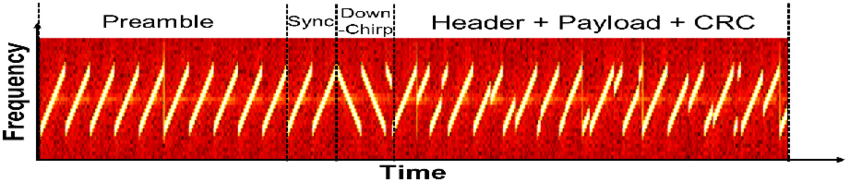
\includegraphics[width=1\textwidth]{Figures/lora_packet_chirps}
            \caption{Vizualizace odeslaného LoRa paketu --- CSS modulace}
            \label{fig:LoRa_packetvizualisation}
        \end{centering}
    \end{figure}

    Datová struktura paketu je detailněji popsána v \ref{subsubsec:LoRa_Packet}.
    
    U CSS modulace je důležitá tzv. SF hodnota, \textit{Spreading Factor}. 
    Ta určuje sklon jednotlivých 
    chirpů, což ovlivňuje časovou délku jednoho chirpu. Při vyšších
    hodnotách SF je sklon jednotlivých chirpů vyšší, komunikace trvá déle, ale
    je více odolná proti rušení a má vyšší dosah.
    Při nižších hodnotách SF jsou chirpy naopak strmější, čímž je dosaženo vyšší
    komunikační rychlosti, avšak za cenu nižšího dosahu a vyšší náchylnosti k
    zarušení.

    Velkou výhodou CSS modulace je, že se signály s odlišnými hodnotami SF 
    navzájem neruší --- tzn. je možno pro více zařízení komunikovat najednou,
    pokud komunikují odlišnými rychlostmi. Toho využívá ADR mechanismus sítě
    LoRaWAN, který přiděluje nižší rychlosti s vyšším dosahem vzdálenějším
    zařízením a naopak.

    Dalšími výhodami CSS modulace jsou:
    \begin{itemize}
        \item Odolnost proti Dopplerově efektu (změna frekvence v případě pohybu 
            vysílače či přijímače)
        \item Odolnost proti rušení vzniklému přijetím signálů šířících se od
            vysílače různě dlouhými cestami
        \item Vysoká hodnota link budget --- tzn. vysoká citlivost přijímače na
            slabé signály pod hladinou okolního šumu
    \end{itemize}

    %Obrázek z https://www.researchgate.net/figure/
    %LoRa-packet-structure_fig1_316999094

\section{Použité frekvence}

    LoRa funguje na sub-GHz bezlicenčních frekvencích, tzn. v ISM pásmech. 
    V České republice jsou k dispozici pásma EU433 a EU868. Název EU868 se 
    používá pro pásmo 863-870 MHz, které je v ČR pro LoRu běžně používáno. 
    Toto pásmo je definováno normou ETSI EN300.220, informace k němu lze také 
    najít v dané normě odpovídajícímu všeobecném oprávnění č. VO-R/10/12.2019-9
    vydaném českým telekomunikačním úřadem.

    Další informace k použitým frekvencím a kanálům jsou uvedeny v tabulce
    \ref{tab:LoRaWAN_datarates}.

%https://lora-alliance.org/sites/default/files/2018-07/lorawan\_regional\_%
%parameters\_v1.0.3reva\_0.pdf

%https://www.ctu.cz/sites/default/files/obsah/ctu/vseobecne-opravneni-c.vo-r%
%/10/12.2019-9/obrazky/vo-r10-122019-9.pdf

\section{LoRa packet}
    \label{subsubsec:LoRa_Packet}

    Data jsou vysílána v paketech. Součástí paketu jsou vždy preambule, 
    samotná data a kontrolní CRC součet dat ,
    Navíc může být přítomna hlavička a její kontrolní CRC součet.
    Délky jednotlivých částí paketu jsou proměnné. 
    
    Hlavička obsahuje parametry komunikace, zejména pak hodnotu CR (popsána v \ref{sec:FEC}), délku 
    přenášených dat a informaci o tom zda je přítomný 
    CRC součet přenášených dat. 
    
    LoRa rozlišuje dva typy paketů:

    \begin{description}
        \label{lst:LoRa_packet_types}
        \item [Explicitní] pakety obsahují všechny výše uvedené informace
        \item [Implicitni] pakety neobsahují hlavičku. Lze je použít, pokud jsou
            informace obsažené v hlavičce příjemci předem známy
    \end{description}

    Implicitní pakety lze používat, jsou-li informace v hlavičce uvedené 
    přijímací straně předem známy.

    Na obrázku \ref{fig:LoRa_packet_structure} lze vidět jednotlivé části
    paketu. Je z něj také patrné, že zatímco hodnota SF je pro celý paket 
    konstantní, hodnota CR se může lišit mezi hlavičkou a daty --- pro hlavičku je
    pevně stanovena, pro data je uvedena v hlavičce.

    \begin{figure}[h]
        \begin{centering}
            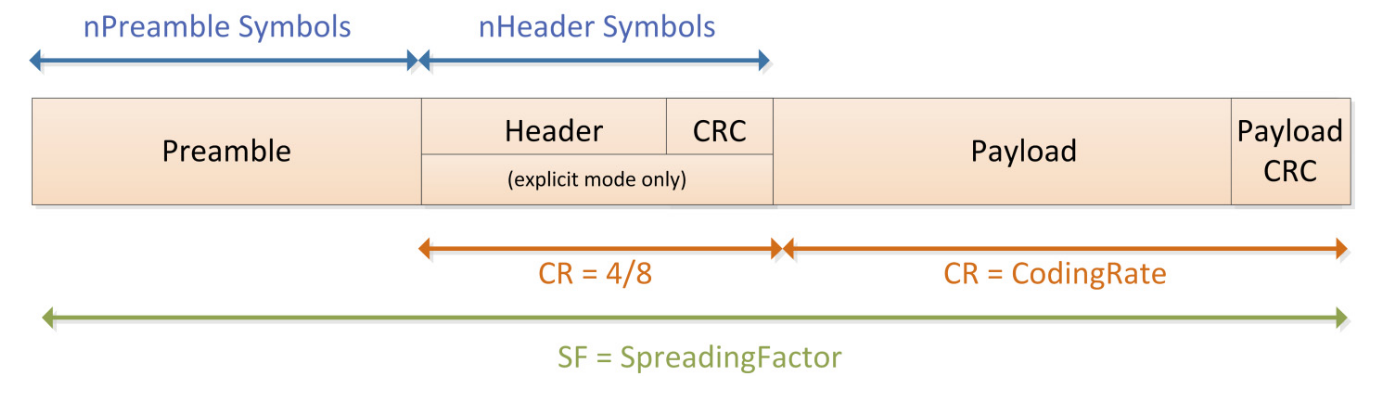
\includegraphics[width=1\textwidth]{Figures/lora_packet_structure}
            \caption{Struktura LoRa paketu}
            \label{fig:LoRa_packet_structure}
        \end{centering}
    \end{figure}

% Obrázek z datasheetu SX1261

\section{Forward Error Correcting}\label{sec:FEC}

    LoRa využívá dopřednou korekci chyb. Ta spočívá v doplnění korekčních bitů
    k odeslaným datům. Oproti např. běžně užívaným paritním bitům umožňují
    korekční bity nejen detekci chyb, ale také do jisté míry jejich korekci na
    straně přijímače, bez nutnosti opakovaného zaslání celé zprávy či jejích
    částí.

    Množství doplněných korekčních bitů je volitelné --- jejich vyšší množství
    poskytuje vyšší robustnost komunikace, avšak za cenu vyššího nárůstu
    celkového množství odeslaných dat.

    Množství korekčních bitů je určeno parametrem Coding Rate. Ten se udává ve 
    formě poměru dvou čísel, obvykle v rozmezí 4/5 až 4/8. Např. u poměru 4/5 
    se na každé 4 bity uživatelských dat se přidá jeden korekční bit, u poměru
    4/7 se přidají tři korekční bity atp.

    Tabulka níže uvádí běžné hodnoty poměrů užívané při LoRa komunikaci, a 
    jejich označení hodnotou CR.

    \begin{table}
        \begin{centering}
            \caption{Možnosti dopředné opravy chyb SX1261}
            \begin{tabular}{|>{\centering}p{0.25\textwidth}|>{\centering}
                    p{0.25\textwidth}|>{\centering}p{0.25\textwidth}|}
                \hline 
                Číselné označení použité korekce --- CR, Coding Rate
                & Poměr mezi datovými bity a korekčními bity 
                & Nárůst množství dat po doplnění korekčních bitů
                    \tabularnewline
                \hline 
                \hline 
                1 & 4/5 & 1,25\tabularnewline
                \hline 
                2 & 4/6 & 1,5\tabularnewline
                \hline 
                3 & 4/7 & 1,75\tabularnewline
                \hline 
                4 & 4/8 & 2\tabularnewline
                \hline 
            \end{tabular}
        \par
        \end{centering}
    \end{table}